%%%%%%%%%%%%%%%%%%%%%%%%%%%%%%%%%%%%%%%%%%%%%%%%%%%%%%%%%%%%%%%%%%%%%%%%%%%%%%%
% Generative AI
%%%%%%%%%%%%%%%%%%%%%%%%%%%%%%%%%%%%%%%%%%%%%%%%%%%%%%%%%%%%%%%%%%%%%%%%%%%%%%%

\section{Generative AI}
\label{sec:generative-ai}

This section explores the growing influence of \textit{generative artificial intelligence} (GenAI), particularly in the form of \textit{large language models} (LLMs), on programming fundamentals pedagogy and software development practice. While the broader implications discussed here apply to most textual programming languages, the focus is primarily Python-based education, with a particular emphasis on creative coding and the generation of visual output where possible.

GenAI is a vast and rapidly evolving field; given its breadth and complexity, any single facet could warrant an entire doctoral investigation. Accordingly, this section provides a high-level overview, focusing on aspects most relevant to this PhD study. It aims to establish a conceptual foundation for subsequent references to GenAI, particularly in the context of assessment design and future research direction for this work.

\textbf{This section is a late-stage addition to the PhD, included to address significant developments that rose to prominence during the candidature.} At commencement (2018/2019), GenAI had minimal impact on programming education. Since 2022, however, tools such as ChatGPT and GitHub Copilot have significantly reshaped how programmers, educators, students, and artists engage with code and creative expression~\cite{world_intellectual_property_organization_generative_2024}. These technologies have introduced both opportunities and challenges, prompting a widespread re-evaluation of pedagogy, assessment design, and ethical frameworks~\cite{odea_generative_2024}. Had such tools been available at the outset, this PhD may have followed a markedly different trajectory. Nonetheless, its contributions remain novel, spanning new pedagogical strategies, software tools, and learning materials that may complement or integrate with emerging GenAI-supported teaching practices.

In addition to surveying existing literature, this section incorporates brief, illustrative demonstrations using GenAI tools such as Builder.io, ChatGPT, and Replit Agent. While not formal studies, these exploratory examples serve as practical complements to the literature, helping to contextualise published research. This approach reflects Torraco's conception of integrative literature reviews, which may include limited empirical samples to probe, validate, or challenge existing knowledge~\cite{torraco_writing_2005}.

Preliminary trials using Thonny-py5mode suggest that creative coding tasks---specifically those requiring students to generate visual output through code---may offer some resistance to unauthorised GenAI assistance. This ancillary insight arose during the study reported in the article \textit{\nameref{sec:jise}}, which examined students' use of Thonny-py5mode for visual coding challenges. While this appears to be a promising way to mitigate GenAI cheating, it is an early finding. Moreover, its effectiveness is likely limited to a few years (perhaps less) given the rapid evolution of GenAI tools~\cite{ganguli_predictability_2022, grace_viewpoint_2018}. As GenAI is not the primary focus of this research or the aforementioned article, these insights are presented as complementary, extending the literature review on assessment practices in the GenAI era in line with Torraco's integrative framework.

This section opens with an overview of code generation using GenAI to highlight its current capabilities. It then explores GenAI's growing role in introductory programming education, particularly recent debate around and proposed shifts in teaching and assessment. The discussion concludes with the experimental work using visual coding tasks as a potential mitigation strategy against students' misuse of GenAI to complete assessment tasks.

\subsection{Generating Code Using GenAI}
\label{subsec:generating-code-using-genai}

GenAI refers to a broad and rapidly evolving class of artificial intelligence models capable of generating new content based on patterns learned from data. These outputs span a wide range of modalities, including text, code, images, music, video, 3D models, speech, animations, video game levels, and data simulations~\cite{foo_ai-generated_2025}. Among GenAI technologies, Large language models (LLMs) specialise in producing human-like text. Because programming code is inherently textual and follows a constrained logical structure, LLMs can also generate partial or complete scripts in languages such as Python. This capability is sometimes labelled \textit{LLM-driven program synthesis}~\cite{austin_program_2021}.

Users interact with LLM-powered code generation tools in several ways, including: \textbf{conversational prompting}, which involves describing coding requests through chat interfaces and engaging in iterative dialogue to refine requirements; \textbf{inline code completion}, as seen in tools like GitHub Copilot that provide real-time suggestions while typing in IDEs; and \textbf{code explanation and documentation}, where users highlight existing code to receive explanations, generate comments, or produce documentation. Additionally, GenAI technologies can facilitate code translation across languages and paradigms, assist with testing and validation, and streamline development workflows through intelligent automation and tooling~\cite{jiang_survey_2024, porter_learn_2024, taulli_ai-assisted_2024}.

Several studies have evaluated the impact of GenAI tools on developer productivity. For example, Peng \textit{et al.} (2023) found that GitHub Copilot significantly improved efficiency, with developers completing a web development task approximately 56\% faster than those in the control group~\cite{peng_impact_2023}. However, its effectiveness appears to be context-dependent. Vaithilingam \textit{et al.} (2022) reported that although developers generally appreciated Copilot as a helpful starting point, it did not consistently lead to faster or more accurate task completion~\cite{vaithilingam_expectation_2022}. Barke \textit{et al.} (2022) observed that developers used Copilot in two primary ways: to accelerate routine tasks and to explore unfamiliar APIs or implementations. While the tool often supported exploratory coding, it occasionally introduced subtle errors requiring careful review~\cite{barke_grounded_2023}. 

More recent Copilot findings, however, reflect improvements in GenAI capabilities, aligning with broader research that demonstrates how increasingly advanced AI models continue to evolve and improve over time~\cite{jiang_survey_2024, huynh_large_2025}. A large-scale study by GitHub and Accenture, published in May 2024, reported that Copilot increased developer speed by up to 55\%, boosted pull request volume by 8.7\%, and improved merge rates by 15\%, alongside an 84\% increase in successful builds. Furthermore, 90\% of developers reported higher job fulfilment, with rapid and sustained Copilot adoption. Specifically, 96\% accepted suggestions on day one, 67\% used the tool at least five days a week, and 95\% said they enjoyed coding more with it~\cite{gao_research_2024}.

Beyond professional programmers, the impact of GenAI is even more pronounced among non-experts. While navigating and operating an IDE with Copilot requires some familiarity with software development, individuals with little to zero programming experience can generate functional code using LLMs such as GPT-4 or Code LLaMA simply by providing natural language prompts~\cite{jiang_survey_2024}. It is important to note, however, that without foundational coding knowledge, such users often struggle to interpret, adapt, or iteratively refine the generated code~\cite{ma_srlcg_2025}.

\subsubsection{GPT-4 Example}

GPT-4 is a large language model developed by OpenAI capable of generating human-like text and functional code in response to natural language prompts. It is most widely accessed through ChatGPT, a conversational interface designed for general users~\cite{openai_gpt-4_2024}. To illustrate its capabilities, consider a simple experiment: a novice user, unfamiliar with programming, prompts ChatGPT to \textit{``write a Python program to add two numbers.''} Testing this in June 2025, the model returns the following script:

\begin{lstlisting}
# Program to add two numbers

# Input from user
num1 = float(input("Enter first number: "))
num2 = float(input("Enter second number: "))

# Add the two numbers
sum = num1 + num2

# Display the result
print("The sum is:", sum)
\end{lstlisting}

In this example, the LLM generates output that is correct, functional, and consistent with PEP 8, the widely accepted style guide for Python~\cite{van_rossum_pep_2013}. While the script is syntactically simple, a novice may still struggle to iteratively refine (or even run?) it. Even minor adaptations---such as handling integers, adding operands, or rounding output---require a working knowledge of expressions, variable assignment, and built-in functions. Adding error handling for invalid inputs further assumes familiarity with control flow and debugging, while running the script itself presupposes some understanding of terminal environments.

Of course, one could prompt further such refinements, but this introduces a different kind of dependency: rather than learning to reason about code, the novice may become reliant on iterative prompting as a substitute for conceptual understanding. This risks promoting surface-level engagement, where the user treats the model as a `black box' capable of correcting or rewriting code on demand, without necessarily grasping the logic behind it. In educational contexts, this pattern raises concerns about the erosion of foundational programming skills and the challenge of distinguishing between genuine comprehension and GenAI-enabled mimicry by learners~\cite{kazemitabaar_studying_2023}.

Prather \textit{et al.} investigated the differential impact of GenAI tools on novice programmers and found that such technologies tend to amplify existing disparities rather than mitigate them. In their study, students with higher prior performance and self-efficacy were able to leverage GenAI to accelerate their progress, often using it strategically to test ideas or refine code. In contrast, students who were already struggling relied on it in ways that masked their lack of understanding, leading to superficial task completion without deeper learning~\cite{prather_widening_2024}. 

Kiesler \& Schiffner (2023) demonstrate that GPT-4 performs strongly on beginner programming tasks, solving 94.4\% correctly. The study used 72 appropriately-scoped Python tasks from CodingBat\footnote{~\url{https://codingbat.com/python}}, typical of CS1 courses, covering foundational topics like strings, lists, and logic~\cite{kiesler_large_2023}. 

However, LLMs are capable of performing tasks far more complex than simple addition scripts or CS1-level assessment work, including the generation and deployment of complete applications. For instance, Replit Agent can create fully functional web apps from a single natural language prompt.

\subsubsection{Replit Agent Example}

Replit Agent scaffolds complete project structures, generates both front- and back-end code, installs dependencies, and supports real-time debugging; this places it among a new class of tools for end-to-end software prototyping. Comparable in ambition to platforms like Builder.io, it allows users to move from concept to deployment with minimal manual setup. Integrated into the web-based Replit IDE with live previews, the Agent enables an iterative, conversational workflow where users can refine and expand their projects through follow-up prompts~\cite{replit_inc_replit_2025}.

Figure~\ref{fig:replit-ai-prompt} presents a simple example designed to evaluate the capabilities of the Replit Agent. The prompt is deliberately crafted to avoid generic projects---such as a shopping cart, to-do list app, or snake-like game---in favour of a more novel and potentially challenging use case. The input reads:

\textit{``Make me an interactive playground for experimenting with Python that helps students understand Turtle,''} with an additional line that states, \textit{``Use a design that appeals to those in creative fields of study.''}

\begin{figure}[!htbp]
\centering
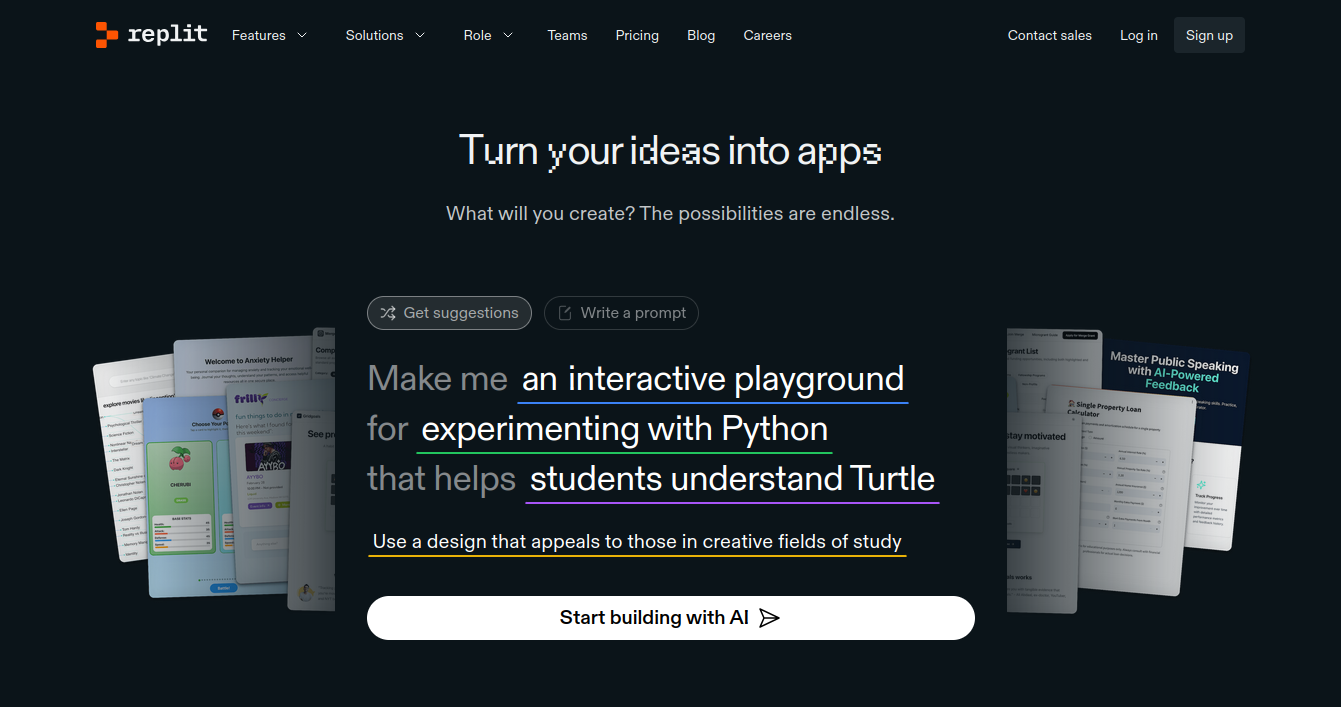
\includegraphics[width=1.0\textwidth]{chapters/chapter02-literature-review/replit-ai-prompt}
\caption{Screenshot (by author) of the Replit Agent prompt interface. Source:~\cite{replit_inc_replit_2025-1}.}
\label{fig:replit-ai-prompt}
\end{figure}

Figure~\ref{fig:replit-ai-result} shows the generated application. It features an integrated code editor, server-side Python execution using Python's built-in \texttt{exec()} function, working Turtle graphics output, and ten curated example sketches, ranging from simple shapes to complex fractals. Each example sketch includes descriptive annotations to support student understanding. Additional elements include canvas controls and a reference section with essential commands (at the foot of the page), among other `thoughtful' (yet unprompted) design elements.

\begin{figure}[!htbp]
\centering
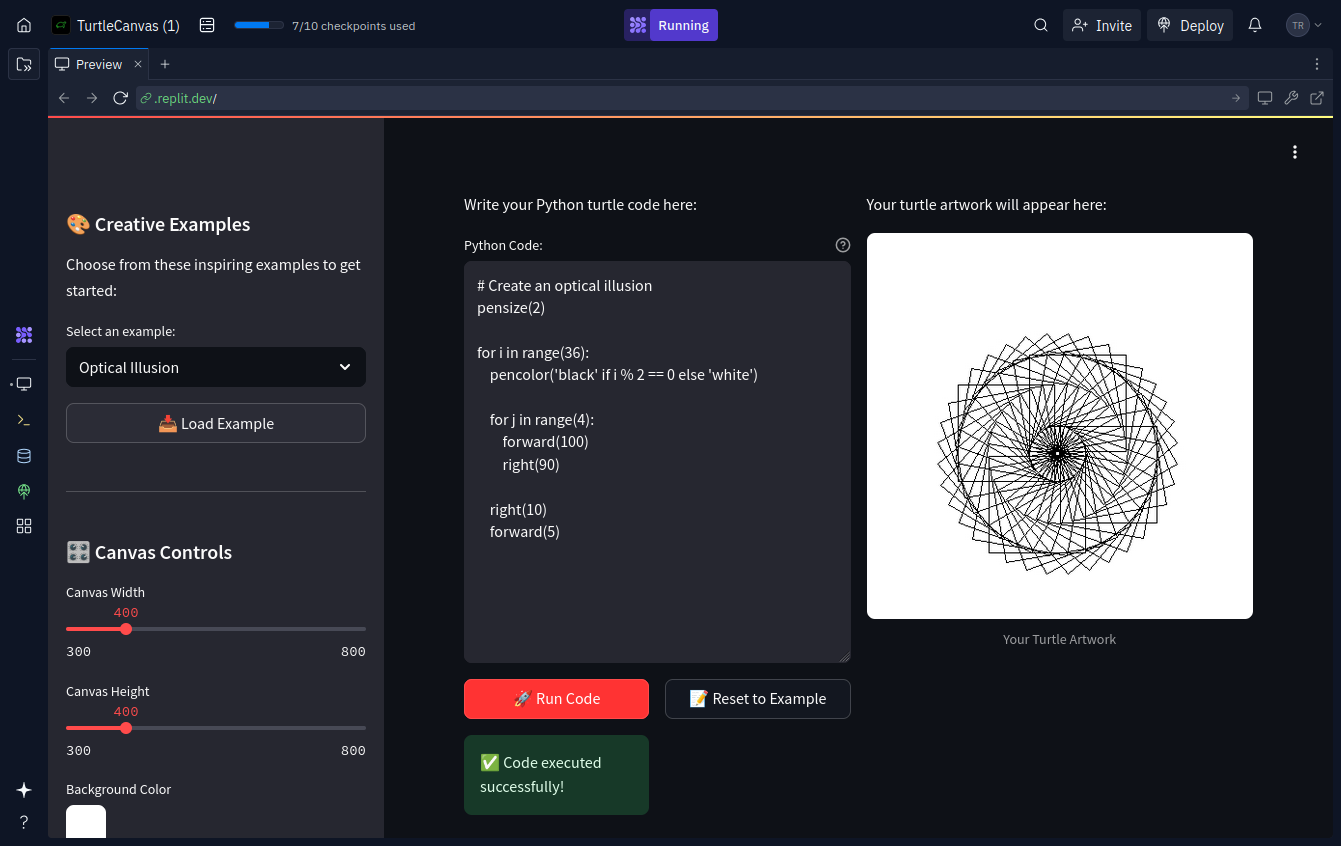
\includegraphics[width=1.0\textwidth]{chapters/chapter02-literature-review/replit-ai-result}
\caption{Turtle app generated using a Replit Agent prompt (see Figure~\ref{fig:replit-ai-prompt}). Screenshot of the deployed result on replit.com. Source:~\cite{replit_inc_replit_2025-2}.}
\label{fig:replit-ai-result}
\end{figure}

All key features of the application function as expected, though there are limitations and areas for refinement. For instance, the \textit{Print} option under the `kebab' menu produces a disjointed layout, scattering interface elements across multiple pages rather than formatting them on a single printed page. Printing the user's Turtle code alongside the corresponding graphic output would arguably better meet user expectations. That said, the Agent's chat-like interface allows for iterative prompting, and with some refinement, the printed arrangement can be improved.

Further analysis of the generated code revealed that the application is built using Streamlit, a Python-based framework that abstracts away traditional front-end development. The conventional prefix for using Streamlit in Python is \texttt{st}. Streamlit automatically generates the HTML and CSS required to render a functional web interface, handling the layout components, user-input widgets, and some visual styling. For example, calling \texttt{st.slider()} or \texttt{st.button()} in Python produces appropriately styled HTML elements with built-in interactivity and responsive design. As a result, the project contains no separate HTML, CSS, or JavaScript files. It comprises approximately 656 lines of Python code, distributed as follows:

\begin{itemize}
  \item \textbf{193 lines} for the main Streamlit interface (\textit{app.py})
  \item \textbf{205 lines} for a curated collection of example scripts (\textit{examples.py})
  \item \textbf{258 lines} for the underlying Turtle graphics engine (\textit{turtle\_engine.py})
\end{itemize}

This example, along with recent literature~\cite{day_get_2025, gadde_democratizing_2025, sapkota_vibe_2025} highlights the growing potential of LLM-driven development environments to support comprehensive software prototyping workflows. In this instance, Replit Agent demonstrates how a concise prompt can yield a functional, multi-file Python application with a coherent interface, making intuitive decisions about UI components, technical architecture, and additional features without explicit instruction.

\subsubsection{Builder.io Comparison}

To further investigate the capabilities of natural language to code, Figure~\ref{fig:builder.io-result} presents the result of a Builder.io experiment using the same prompt: \textit{''Make me an interactive playground for experimenting with Python that helps students understand Turtle.''} While Builder.io produced a web app with functional core features, the interface exhibited several unstable elements, and the application became unresponsive after loading a few code examples.

\begin{figure}[!htbp]
\centering
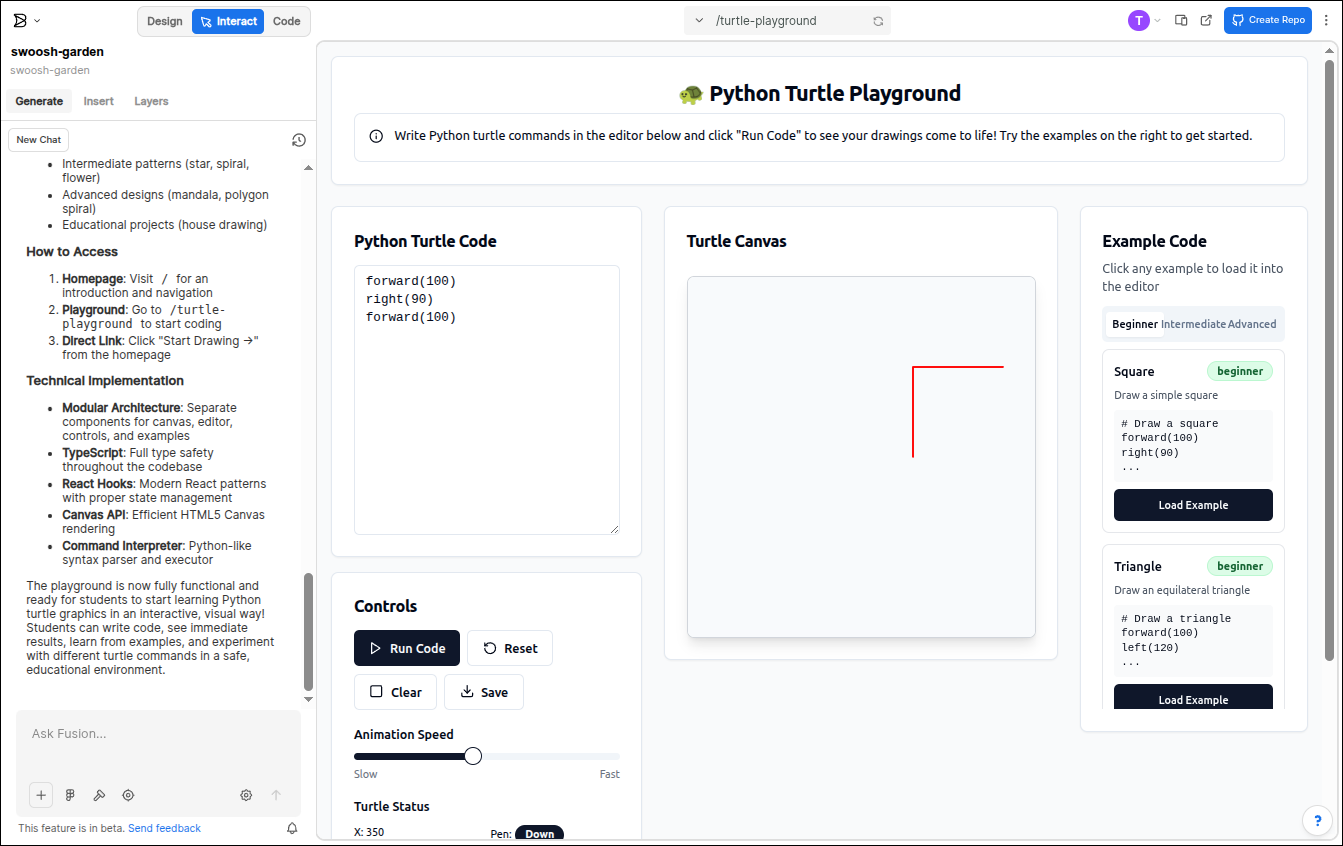
\includegraphics[width=1.0\textwidth]{chapters/chapter02-literature-review/builder.io-result}
\caption{Result generated by Builder.io in response to the prompt: \textit{``Make me an interactive playground for experimenting with Python that helps students understand Turtle.''} Screenshot by the author. Source:~\cite{builderio_inc_builderio_2025}.}
\label{fig:builder.io-result}
\end{figure}

Unlike the Replit Agent solution, Builder.io generated a React application written in TypeScript (in contrast to Replit's opting for Streamlit in Python). The project included an integrated code editor powered by Monaco, client-side Python execution via Pyodide, Tailwind CSS for styling, and a comparable set of example sketches. As a result of this architecture, the application code spanned many distinct files and file types (not just a few Python scripts) totalling:

\begin{itemize}
  \item \textbf{502 total lines} for the backend logic (\textit{graphics engine, command interpreter})
  \item \textbf{680 total lines} for the UI (\textit{main playground, example library, controls, editor, canvas})
  \item \textbf{61 total lines} for integration (\textit{route setup, homepage})
\end{itemize}

Further prompting with \textit{``use a design that appeals to those in creative fields of study''} resulted in a more colourful and vibrant interface. However, this also led to further degradation, and it was no longer possible to type Turtle commands into the integrated editor. Additional prompting resolved some of the project's bugs and proved effective in refining some design aspects.

In both instances (Replit and Builder.io), the AI autonomously selected its technical architecture. However, it is entirely possible to prompt Replit to use the same stack as Builder.io and \textit{vice versa}. This demonstrates the flexibility of LLM-based tools when provided with specific guidance. 

In conclusion, while output quality may vary across platforms, implementation specifications, and even between identical prompts, it appears that a broader trend toward natural-language-driven software creation is gaining momentum~\cite{alenezi_ai-driven_2025, osmani_beyond_2025, subramonyam_prototyping_2025}. These Replit and Builder.io examples demonstrate the increasing potential of GenAI-powered development environments to surpass simple code snippets and produce fully structured, functional applications. Again, this convenience could hinder learning, enticing students to overlook essential coding practices, which may foster dependence on generated solutions and detract from developing a deeper understanding of Python programming concepts.

\subsection{GenAI in Introductory Python Education}

LLM technology has sparked the development of multiple GenAI-powered assistance and tutoring tools, along with a growing body of research on their efficacy and application in educational settings. The integration of these technologies, whether instructor-authorised or not, into introductory programming courses marks a significant shift in computing education. Tools such as GitHub Copilot and Codeium Chat enable students to combine natural language and Python as they write code, offering new modes of interaction and enhanced learning support. This has provoked diverse views on whether and how to incorporate GenAI into introductory Python programming curricula.

\subsubsection{GenAI-Powered Programming Assistants}

IDEs and other programming tools are increasingly embedding GenAI-powered features such as live problem assistance, contextual guidance, and conversational prompting~\cite{amiri_enhancing_2025, yang_enhancing_2024, zabala_development_2024}. For instance, Anaconda, a widely used Python distribution, now integrates Anaconda Assistant\footnote{~\url{https://www.anaconda.com/docs/tools/anaconda-notebooks/anaconda-toolbox/anaconda-assistant}} within its Jupyter notebook environments (Figure~\ref{fig:anaconda-ai-assistant})---a popular choice for work focused on data science, machine learning, and interdisciplinary applications of programming. 

\begin{figure}[htbp]
  \centering
  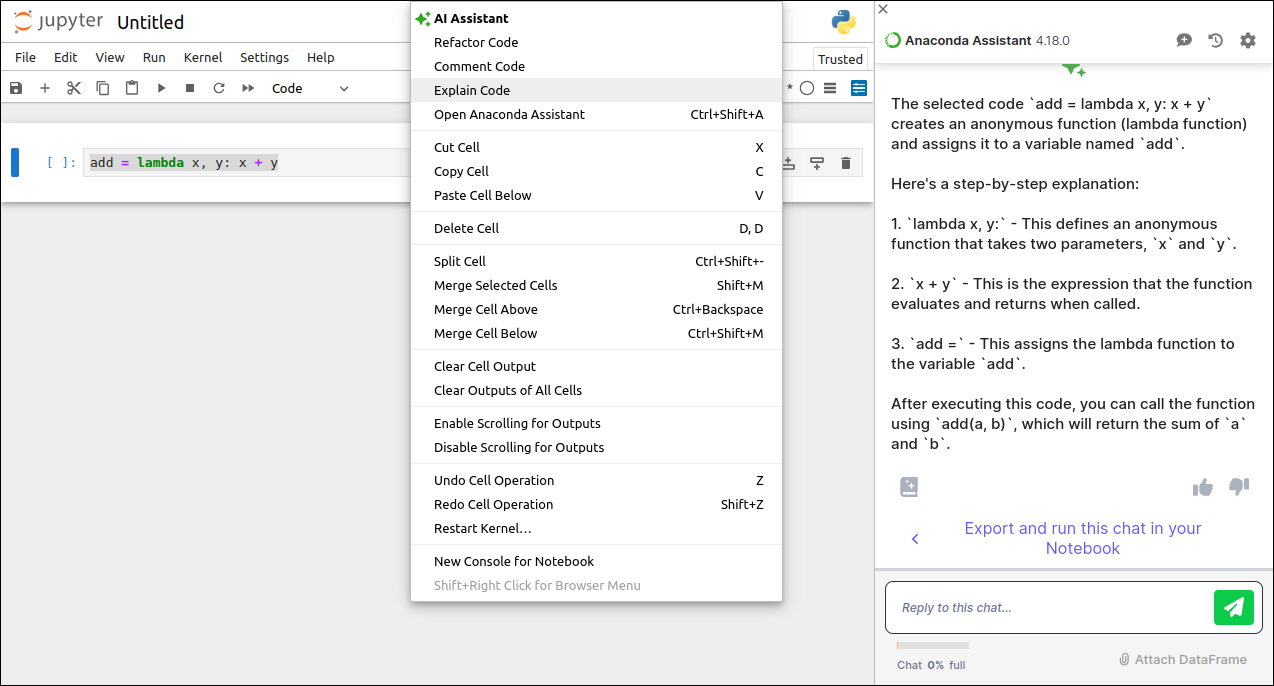
\includegraphics[width=1.0\textwidth]{chapters/chapter02-literature-review/anaconda-ai-assistant}
  \caption{Jupyter Notebook, bundled with Anaconda Navigator (version 2.6.3), used to access the AI Assistant to explain the workings of a \texttt{lambda} expression. Screenshot by the author.}
  \label{fig:anaconda-ai-assistant}
\end{figure}

A notebook coding environment combines executable code cells, narrative text (typically written in Markdown), and graphics (such as charts, tables, and images), allowing users to write and run code in segments, view results inline, and document their process alongside the code and output~\cite{vaughan_python_2023}. While less prevalent in traditional CS1 modules focused on software engineering fundamentals, educators are increasingly adopting notebooks in educational settings that prioritise data science \& analytics, STEM disciplines where code accompanies analysis, and literate programming\footnote{~\textit{Literate programming} is a programming paradigm introduced by Donald Knuth (1984) that emphasises writing code as an explanation intended for humans first and computers second. It blends natural language narrative with source code, allowing the author to describe the logic, reasoning, and intent alongside functional code~\cite{rule_ten_2019}.} contexts~\cite{bascunana_impact_2023, johnson_benefits_2020, yavuz_temel_using_2025}.

Despite the limitations of GenAI and concerns surrounding its use in education, studies confirm its potential for supporting learners. Recent research suggests that tools like ChatGPT and Anaconda's AI assistant can aid students learning Python, providing helpful on-demand assistance for debugging, concept clarification, and syntax correction~\cite{liu_teaching_2024, yang_enhancing_2024}. 

Phung \textit{et al.} conducted benchmarking studies showing that GPT-4 approaches the performance of human tutors in tasks such as program repair, hint generation, and contextualised explanation for introductory coding problems. Their study demonstrates that GenAI models can serve in multiple instructional roles, including as a pair programming partner, a source of grading feedback, and a generator of simple practice tasks. However, while models perform well in debugging and explanation, they remain substantially less effective in scenarios requiring deeper reasoning, such as assessing edge-case correctness or synthesising pedagogically appropriate new tasks~\cite{phung_generative_2023}. 

Ouaazki \textit{et al.} utilised the Graasp platform\footnote{~\url{https://graasp.org}}, featuring an integrated GPT-3 chatbot (Graasp Bot), to investigate the role of prompt-tuned GenAI in self-directed computational thinking tasks within an introductory Python course. They found that it proved helpful as a coding assistant in early learning development stages; however, its effectiveness declined with an increase in task complexity. The authors highlighted the need to balance personalisation, usability, and learning depth when integrating GenAI into educational contexts~\cite{ouaazki_generative_2024}.

Scholl and Kiesler (2024) surveyed 298 first-year computer science students, revealing widespread use of ChatGPT-3.5. While students valued the tool for its immediacy and support in Python programming tasks, they also expressed concerns about accuracy, over-reliance, and equitable access. Some students advocated for formally integrating GenAI into computing education, provided it be accompanied by appropriate guidance and safeguards, noting its potential to accelerate learning and reduce cognitive effort~\cite{scholl_how_2024}.

Finally, Moon et al. (2024) conducted a study across four university courses involving 57 students working with p5.js, alongside additional libraries in advanced courses, such as Three.js, Node.js, and ml5.js. The research explored how conversational AI tools, including ChatGPT and GitHub Copilot, support creative coding education. The findings echoed broader trends in GenAI-assisted programming: while beginners benefited from real-time feedback, debugging help, and code generation, it was advanced students who used GenAI most effectively to experiment and learn. Less experienced students often struggled with crafting effective prompts, misinterpreted output, and were more prone to over-reliance on generated code~\cite{moon_teaching_2024}.

\subsubsection{GenAI-Powered Tutoring Systems}

The boundary between general-purpose coding assistants and intelligent tutoring systems (ITSs) is becoming increasingly blurred. ITSs are designed to emulate human tutors by offering adaptive instruction, personalised feedback, task scaffolding, mastery tracking, and interactive problem-solving support~\cite{crow_intelligent_2018}. Meanwhile, GenAI-powered programming assistants---initially developed for tasks like code generation, explanation, and debugging---are beginning to fulfil similar instructional roles, mainly when prompted strategically. For effective learning, however, students must seek hints, scaffolding, or conceptual clarification instead of direct solutions. 

Reflecting this convergence, a new wave of LLM-based software is emerging that explicitly targets educational use. These systems promote deeper engagement by limiting the information they provide, offering partial solutions, step-by-step guidance, or Socratic questioning rather than complete answers. In doing so, they move beyond basic code assistance to deliver pedagogically-informed feedback aligned with learning goals~\cite{chen_gptutor_2023}.

A search of the ACM Digital Library using the query \texttt{"Python" AND ("AI tutoring" OR "intelligent tutoring system")} and filtering for publications between 2022 and 2025 returned over a hundred results. While not all are directly relevant, the volume reflects a surge of recent research at the intersection of programming education and AI tutoring. In contrast, the same query yields far fewer results before 2022, and zero results when narrowed to just \texttt{"Python" AND "AI tutoring"}. This highlights the rapid emergence of interest likely spurred by advances in GenAI. Given that Python remains a dominant language in introductory programming courses~\cite{guo_python_2014}, it is a fitting focus for GenAI-assisted learning.

Yang \textit{et al.} (2024) conducted an 11-week experimental study with 71 non-STEM university students to evaluate PyTutor: a ChatGPT-based ITS designed to support novice Python programmers. The system delivers four types of structured hints---pseudocode, cloze code, basic code, and advanced code---intended to scaffold problem-solving based on constructivist learning and cognitive load theories. They divided participants into an experimental group, which had access to PyTutor, and a control group without. The study results showed that PyTutor significantly improved engagement and performance on coding tasks, particularly among students with weaker programming backgrounds. However, the authors cautioned against excessive reliance on the tool, noting that overuse can lead to diminished learning gains. Additionally, they emphasised the importance of promoting learner autonomy by fostering students' ability to manage their learning and develop independent problem-solving skills~\cite{yang_advancing_2024}.

This PhD, however, focuses specifically on the intersection of Python and \textit{creative computing}, with particular attention to Python programming for generating visual output.

\subsubsection{GenAI-Powered Tutoring Systems for Creative Computing}

ShiffBot\footnote{~\url{https://shiffbot.withgoogle.com}} is a participatory GenAI tutoring experiment co-developed with Daniel Shiffman, a leading creative coding educator well-known for his work with p5.js (JavaScript) and other Processing environments. A prominent figure in the Processing community, Shiffman runs the YouTube channel \textit{The Coding Train}, which has approximately 1.75 million subscribers and over 130 million total views across more than a thousand videos. He is also the author of \textit{Learning Processing} and \textit{The Nature of Code}, and a creator of numerous tutorials and courses related to p5.js~\cite{shiffman_coding_2025}. 

ShiffBot is a Chrome web browser extension that, once installed, appears embedded directly within the p5.js web editor (Figure~\ref{fig:shiffbot}), enabling it to respond contextually to users' code.

\begin{figure}[htbp]
\centering
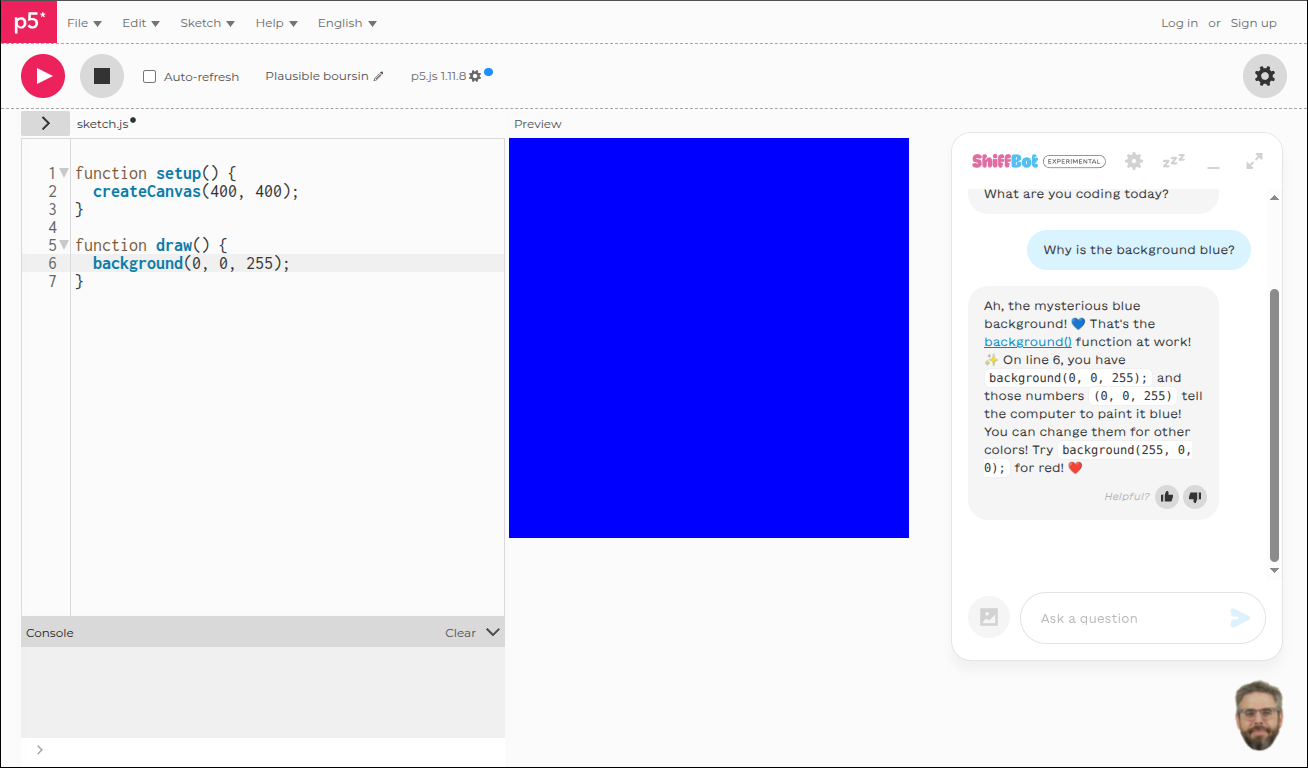
\includegraphics[width=1.0\textwidth]{chapters/chapter02-literature-review/shiffbot}
\caption{Shiffbot, embedded in the p5.js editor, responds to the question ``Why is the background blue?'' Screenshot by the author. Source:~\cite{p5js_contributors_p5js_2025}.}
\label{fig:shiffbot}
\end{figure}

Developed around Shiffman's distinctive teaching materials and style, Shiffbot employs retrieval-augmented generation. The ``RAG'' technique involves two key steps: (1) \textit{retrieval}---fetching relevant information from Shiffman's annotated videos, code walk-throughs, and other instructional artefacts; and (2) \textit{generation}---using an LLM to produce responses grounded in both the retrieved information and the input query. This integration allows ShiffBot to deliver accurate, context-sensitive, and pedagogically aligned support for learners~\cite{rubinovitz_how_2024}. It reflects several key design principles: encouraging learner autonomy instead of providing direct answers, highlighting credible and context-relevant resources, fostering a low-pressure environment for experimentation and error, and aligning responses with learners' immediate needs. Student feedback highlighted ShiffBot's value in enhancing code comprehension, debugging, and reflective thinking without interrupting the learning process~\cite{jurenka_towards_2024}.

Extensive searches across academic databases and search engines yielded no Python-based equivalent to Shiffbot---at least not one specifically designed as a GenAI-powered ITS or learning assistant for graphical output. That said, general-purpose tools like GitHub Copilot and IDE-integrated assistants might offer similar types of support. In some preliminary testing, the Anaconda Assistant, combined with py5's notebook kernel, was able to interpret and generate py5 code fairly well (Figure \ref{fig:anaconda-ai-assistant-py5}). More generally, it handled prompts involving libraries such as Matplotlib and PIL/Pillow with decent accuracy, especially for beginner-level tasks. However, unlike Shiffbot, tools like these depend on students using them constructively, rather than just prompting for quick, one-shot solutions.

\begin{figure}[htbp]
\centering
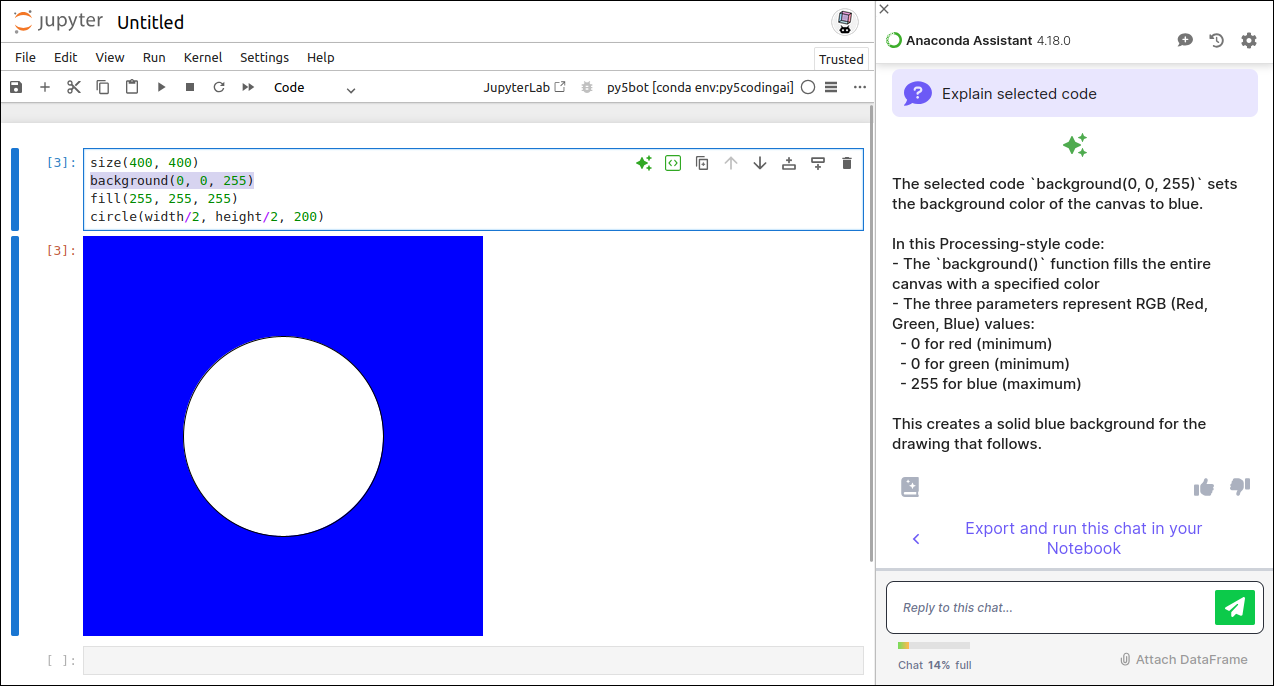
\includegraphics[width=1.0\textwidth]{chapters/chapter02-literature-review/anaconda-ai-assistant-py5}
\caption{py5 running in a Jupyter Notebook, with Anaconda (v2.6.3) Navigator's AI Assistant used to explain the workings of the py5 \texttt{background()} function. Screenshot by the author.}
\label{fig:anaconda-ai-assistant-py5}
\end{figure}

Viewed as a rough technical proof of concept, this py5 + Anaconda Assistant example points toward a promising direction: developing Shiffbot-style tutors tailored to Python-based creative coding. While many GenAI tutors are general-purpose, adapting them to domain-specific pedagogies, especially at the intersection of Python and visual expression, holds growing potential. With multimodal GenAI models, learners could receive feedback on both code and visual output, enabling iterative refinement through conversational interaction. 

In closing, this convergence of GenAI, ITS, and creative coding opens new possibilities for supporting exploratory learning of Python fundamentals through coding graphical output.

\subsection{Mitigating GenAI Misuse}

LLM-powered coding assistants, including conversational tools like ChatGPT, have made it easier than ever for students to generate functional Python code with minimal conceptual understanding of its workings. This can lead to the misuse of GenAI for educational assessments, presenting challenges for educators seeking to uphold academic integrity and accurately assess learners' grasp of Python fundamentals.

The rapid emergence of accessible GenAI tools has prompted colleges and universities to react hastily, resulting in varied strategies across the sector. Some institutions have adopted open, exploratory stances, encouraging students to use GenAI to stimulate creativity, support the development of industry-relevant skills, and enhance learning. In contrast, others have adopted more restrictive policies, citing concerns such as plagiarism, over-reliance on AI-generated code, and the erosion of core programming competencies. In the latter, more regulated environments, GenAI use is often discouraged or explicitly prohibited, particularly in assessments designed to prioritise independent work and originality~\cite{mcdonald_generative_2025}. Nonetheless, enforcing these restrictions is difficult. Among other challenges, educators face limited time and insufficient institutional support to thoroughly investigate suspect submissions. Additionally, existing tools that automate the detection of GenAI content are not entirely reliable, risking the misidentification of legitimate student work~\cite{an_investigating_2025}. 

Some institutions have instead deferred to individual departments or educators, allowing them to set expectations regarding GenAI assistance at the course or even module level. However, this decentralised approach can result in fragmented student experiences, even within the same (diploma/degree) programme. Learners often encounter differing, and sometimes conflicting, expectations depending on their instructor, discipline, or overarching departmental policies~\cite{habel_anusas_2025, trinity_college_dublin_using_2025}.

Within creative computing, some courses formally incorporate GenAI into curricula, encouraging students to explore emerging forms of computational expression. For instance, \textit{Creative Coding and Generative AI} at Carleton College is a project-based course that engages students in creative coding using tools such as Inform~7, Tracery, p5.js, and ml5.js---blending narrative, visuals, code, and AI~\cite{salter_dgah_2025}. Similarly, Victoria University of Wellington offers \textit{Creative Coding and AI}, which integrates GenAI to support both design workflows and code review processes~\cite{victoria_university_of_wellington_dsdn_2025}.

It is also relevant to note that programming visual output with Python provides a tangible way for students to explore the mechanics underlying AI through graphics, animations, and visualisations. For example, Daniel Shiffman's \textit{The Nature of Code} includes chapters on evolutionary algorithms and neural networks, demonstrating concepts using p5.js---approaches that educators can readily adapt to Python using py5 or other Processing-inspired frameworks~\cite{shiffman_nature_2024}. Similarly, Tariq Rashid's \textit{Make Your Own Neural Network} provides an accessible, step-by-step introduction to implementing a neural network in pure Python, which might also be repurposed within graphical or creative coding contexts~\cite{rashid_make_2016}.

GenAI tools continue to evolve; at the same time, they are becoming increasingly embedded in professional workflows~\cite{gao_research_2024, gillespie_trust_2023}. Institutions must face the dual challenge of fostering innovation and adequately preparing students for the industry, while simultaneously safeguarding academic integrity and ensuring adequate foundational learning. Many educators agree that students should engage with GenAI in an ethical, critical, and constructive manner, aligning its use with meaningful learning outcomes. However, this is challenging to ensure.

While GenAI presents significant challenges for assessing student learning, this research contends that its use in Python programming can be permitted---\textit{provided} educators adopt thoughtful assessment design and enforce clear institutional policies to mitigate misuse. Research indicates that a layered approach, combining multiple methods for ensuring academic integrity, can strengthen confidence in the authenticity of student work~\cite{mahon_guidelines_2024}. Given this PhD's focus on Python programming, the discussion categorises mitigation strategies into three groups aligned with programming-specific contexts: \textit{\nameref*{sec:code-tracking-&-authorship-methods}}; \textit{\nameref*{sec:integrity-culture-&-student-engagement}}; and \textit{\nameref*{sec:assessment-design-&-expository-practices}}. These lead to an exploration of Thonny-py5mode as a practical tool for mitigating GenAI misuse through Python-based graphical coding tasks.

\subsubsection{Code Tracking \& Authorship Methods}
\label{sec:code-tracking-&-authorship-methods}

Several strategies directly analyse or track code itself to detect or deter unauthorised GenAI use, reviewing aspects such as its structure, development history, and authorship patterns. 

For instance, \textit{stylometric} techniques treat code as a form of `personal expression,' extracting features such as AST\footnote{An Abstract Syntax Tree (AST) is a simplified, tree-like representation of a computer program's structure~\cite{scott_programming_2016}.} patterns, node type distributions, line lengths, and whitespace conventions to train machine learning models that can distinguish between human and AI authors---or even attribute work to specific individuals. Stylometric analysis can remain effective even after removing superficial cues, though its reliability diminishes with deliberate obfuscation or style imitation~\cite{gurioli_is_2024, idialu_whodunit_2024}. 

In contrast, AI content detectors such as GPTZero and Originality.ai process input as natural language. These are the tools commonly used to evaluate student essays by employing linguistic metrics such as burstiness and perplexity to estimate the likelihood of GenAI authorship. However, this approach is not designed for analysing source code and tends to perform poorly, and often yields false positives, particularly with short or edited Python samples~\cite{grammarly_inc_how_2025}. If employed at all, it is advisable to use such detectors in conjunction with code-specific methods, such as stylometric analysis.

By design, traditional plagiarism detection tools such as MOSS and JPlag do not identify AI-generated content \textit{per se}. However, they remain helpful in flagging clusters of near-identical submissions. Despite the inherent variability of LLM outputs, these clusters often reflect shared prompts or reused AI-generated material, and can assist auditors when interpreted in conjunction with other forms of evidence~\cite{hoq_detecting_2024}.

A more direct strategy involves logging code development history. Tools like GitHub Classroom or IDE-integrated trackers (e.g., zyBooks' Coding Trails) can capture the timing and sequence of edits. Features such as playback or diff visualisations make it easier to identify sudden jumps in progress, large late-stage commits, or other suspicious patterns~\cite{vahid_chatgpt_2023}. Assessment design also plays a key role: requiring staged deliverables (pseudocode, intermediate drafts, and final implementations) encourages incremental work and makes abrupt changes easier to detect~\cite{xie_ai_2023}.

In high-stakes contexts, secure exams administered online or in physically proctored settings remain among the most effective deterrents to cheating. A newer class of online proctoring tools, including platforms such as ProctorU, Honorlock, and Proctorio, employs a range of mechanisms to maintain exam integrity. These typically include webcam and screen monitoring, browser lockdown to prevent tab switching or unauthorised access, ID verification, session recording, and the use of AI and/or human invigilators to flag suspicious behaviour, such as gaze aversion or unusual background noise. While not explicitly designed for coding assessments, their use is increasingly common in Python and other programming exams~\cite{mahon_guidelines_2024}. It is, however, important to acknowledge that such systems raise ethical concerns; this includes surveillance overreach, invasive data collection, algorithmic bias, and restrictions on students' control over their physical space and movement~\cite{lee_online_2022}.

\subsubsection{Integrity Culture \& Student Engagement}
\label{sec:integrity-culture-&-student-engagement}

These strategies do not focus on code itself; instead, they shape student attitudes and behaviours around academic integrity and the responsible use of GenAI, aiming to establish clear and specific policies that promote the ethical use of these tools. 

To support this goal, educators must provide students with explicit guidance on which tools are permitted, under what conditions, and clarification on what constitutes misuse. Where GenAI use is allowed, there are clear guidelines for citation and attribution, communicated along with the consequences of misuse or misattribution. To reinforce these guidelines, learning materials and assessment briefs can incorporate honour pledges and integrity quizzes, ideally integrated into online submission systems and assignment coversheets. Classroom discussions provide another avenue for encouraging individual responsibility, where educators can use these sessions to prompt students to reflect on their values and align their behaviour with institutional expectations~\cite{an_investigating_2025}. 

It is also crucial to explain the rationale behind assessments. Framing these tasks as opportunities for growth rather than as hurdles helps students understand that GenAI misuse undermines their learning and leaves them ill-prepared for real-world technical interviews or practical problem-solving. Encouraging help-seeking through reminders about office hours, peer collaboration, or tutoring services can address pressures that sometimes drive dishonest behaviour~\cite{balalle_reassessing_2025}.

Demonstrating how detection tools operate can serve as a deterrent, raising awareness among students that inappropriate use of GenAI is detectable. Strategic reminders, particularly before assessment deadlines or at key academic milestones, help maintain integrity expectations and reduce the likelihood of students claiming uncertainty about acceptable practices. Perhaps more importantly, there are structured and supervised opportunities for students to engage in ethical GenAI practice. This could involve in-class activities and discussions, as well as critically evaluating the output of different GenAI tools to highlight their potential and limitations. These experiences promote digital literacy and build trust, while shifting the conversation away from fear and toward responsible participation in an evolving technological landscape~\cite{king_artificial_2025}.

\subsubsection{Assessment Design \& Expository Practices}
\label{sec:assessment-design-&-expository-practices}

These strategies reconfigure assessment, requiring students to complete tasks that are more personalised, individualised, expository, or thoughtfully constrained to resist GenAI misuse.

Personalised Python tasks---such as working with self-collected data, generating outputs tied to individual interests, or embedding contextual knowledge---make it more difficult for students to coax useful, one-shot output from GenAI tools. Even with GenAI assistance, such tasks typically require more effort and problem-solving to adapt AI-generated content in a meaningful way~\cite{xie_ai_2023}. 

Assignments tied to current events or newly released APIs can exploit knowledge gaps in GenAI training data. Bespoke datasets introduce contextual dependencies unlikely to be represented in public models~\cite{rahe_how_2025}. Parameter variation, where each student receives a unique dataset or task specifications, further reduces the risk of shared or copied code~\cite{deitrick_individualizing_2022}. Instructors may also redesign tasks to emphasise higher-order thinking and minimise rote GenAI use, focusing on problem-solving rather than implementation details (where GenAI tends to excel), or incorporating more analytical and open-ended requirements~\cite{zastudil_generative_2023}.

Expository strategies, such as reflective writing or recorded walkthroughs, can expose discrepancies between claimed and actual code authorship~\cite{mahon_guidelines_2024}. However, it is important to keep in mind that GenAI tools can generate plausible reflective statements. Nevertheless, students may not always thoroughly review or fully understand these reflective accounts, which can lead to inconsistencies and highlight potentially suspect narratives. Targeted viva-style interviews can help probe understanding when GenAI misuse is suspected, as students who rely on AI often struggle to explain bugs, justify design choices, or narrate their development process~\cite{moorhouse_generative_2023}. Even short reflective questions integrated into submission workflows can interrupt copy-paste habits and reposition coding as a process of cognitive engagement, rather than a deliverable to complete.

Scaffolded deliverables, requiring the incremental submission of early drafts and planning through to final implementation, can further limit the viability of last-minute reliance on GenAI. Complementary approaches, such as code review and debugging exercises, shift the focus from generation to judgment, requiring critical analysis over superficial synthesis. Conducting assessment sub-tasks during lab sessions, in timed settings, or on paper provides controlled conditions for real-time validation of ability. Notably, however, live coding tasks can demand additional resources and may disadvantage students with test anxiety or disabilities. Peer-generated challenges and structured in-class critiques can further promote accountability, requiring students to justify their decisions and engage with others' work~\cite{beaton_instructional_2024}. However, as noted in \nameref{sec:integrity-culture-&-student-engagement}, the effectiveness of these measures depends heavily on class culture and student honesty.

In summary, most strategies present trade-offs. Utilising technical tools, innovative assessment design, and clear policies, along with fostering an integrity-based culture, are essential components of a multi-layered approach to mitigating GenAI misuse in introductory programming assessments. Automated systems can raise accuracy and privacy concerns; high levels of manual oversight may increase instructor workload and still negatively affect the student experience. In reality, determined cheaters may continually adapt to new countermeasures, not to mention employ pre-GenAI techniques that remain effective today, including code sharing, contract cheating, and collusion. Educators should combine technical solutions with open support and a culture that prioritises honesty and learning, striking a balance between encouragement and enforcement.

Drawing from insights primarily in \nameref{sec:assessment-design-&-expository-practices}, the following section outlines an assessment design technique that mitigates GenAI misuse through Python-based graphical coding tasks.

\subsection{Graphical Programming Tasks to Mitigate GenAI Misuse}

Tools like ChatGPT and GitHub Copilot can now solve text-based Python tasks with minimal human understanding, especially those with well-defined instructions and canonical solutions. As GenAI grows ever more capable of reliably producing correct scripts, educators may shift their focus from code production to code interpretation, debugging, and modification. For example, Denny \textit{et al.} challenge students to write prompts for an LLM to generate code that solves a given problem, rather than writing the code themselves~\cite{denny_prompt_2024}. Alternatively, educators might `double down' on hands-on coding practice to reinforce core concepts and facilitate problem-solving resilience. While there is no clear consensus, there is broad agreement that ignoring GenAI's influence is no longer a viable option.

McDanel and Novak (2025) evaluated the performance of LLMs (GPT-3.5, GPT-4o, and Claude Sonnet) on a set of representative, multi-part Python programming tasks from the SIGCSE Nifty Assignments\footnote{~\url{http://nifty.stanford.edu}} set. Their study analysed both qualitative and quantitative aspects of model performance, and proposed practical strategies to help educators design assignments that resist trivial automation by GenAI. The authors explicitly note that ``certain assignments, particularly those involving visual elements, proved challenging for all models.'' Furthermore, they observed that ``when the input is an image or the solution is defined as a correct-looking visual, current era LLMs literally do not have a way to interpret such information and struggle.'' However, ``due to the fuzzy nature of correctness often found in graphical programs, they are usually less testable as well.''~\cite{mcdanel_designing_2025}

Specifically, McDanel and Novak found that a \textit{Sankey Diagrams} assignment using a custom Python library most consistently tripped up LLMs (Figure \ref{fig:nifty-spectrum}), which hallucinated invalid function calls and failed to revise code correctly.

\begin{figure}[htbp]
\centering
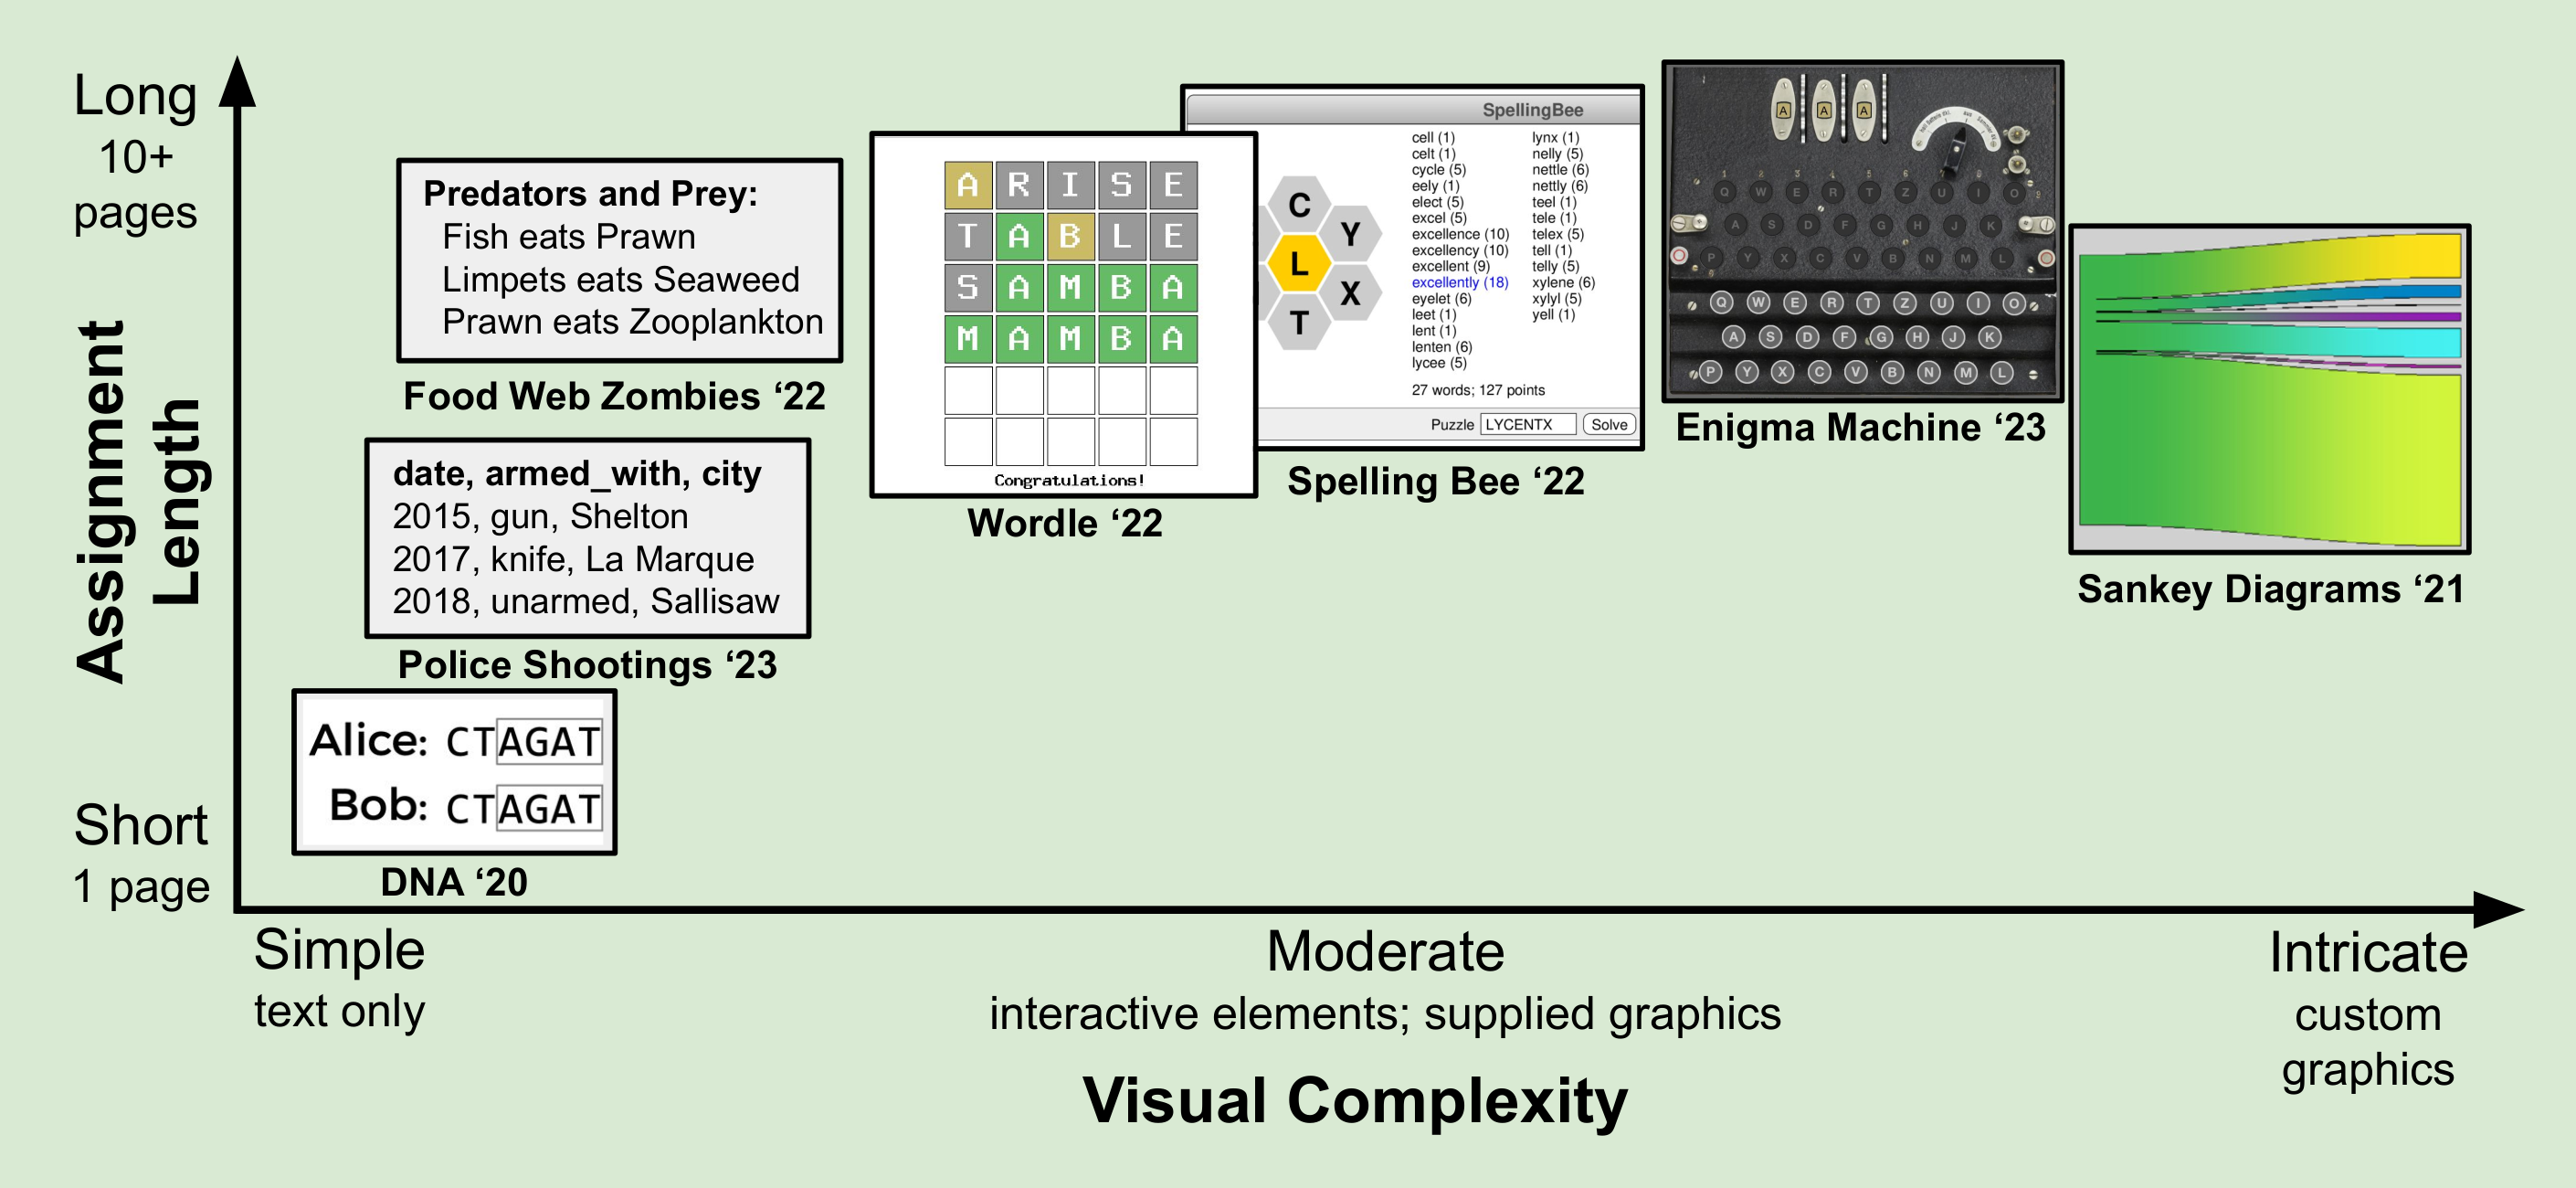
\includegraphics[width=1.0\textwidth]{chapters/chapter02-literature-review/nifty-spectrum}
\caption{McDanel and Novak's spectrum of Nifty Assignments plotted across visual complexity and assignment length. Source:~\cite{mcdanel_designing_2025}.}
\label{fig:nifty-spectrum}
\end{figure}

Similarly, tasks that involved a GUI proved more challenging than text-only exercises, suggesting a link between visual complexity and LLM difficulty~\cite{mcdanel_designing_2025}. Inspired by these findings, this section proposes that Thonny-py5mode is well-suited to mitigating GenAI misuse through graphical programming challenges.

\subsubsection{Evaluating GenAI on Visual Programming Tasks}

An ancillary insight emerged while planning the study reported in \textit{\nameref{sec:jise}}---an investigation into Thonny-py5mode's suitability for teaching Python fundamentals through tasks requiring students to recreate graphical programming outputs. In contrast, the present section focuses exclusively on how GenAI systems perform when attempting those same tasks.

During the development of these graphical programming tasks, it became apparent that py5 programming naturally resists unauthorised GenAI assistance. Unlike the typical text-in, text-out paradigm at which large language models (LLMs) excel, these activities demand visual reasoning and geometric logic---skills not readily outsourced to ChatGPT or similar tools. This suggests a potential avenue for mitigating GenAI-enabled shortcuts, though the finding remains preliminary and warrants further investigation.

\textit{ITP122 Introduction to Programming} at Torrens University Australia is a 12-week subject introducing foundational programming concepts using Python, assuming no prior experience. Notably, most students were enrolled in IT diplomas or degrees rather than creative, arts, or design programs. The revised Assessment 2 incorporated the six graphical challenges. The assessment, due in Week 8, followed coverage of the topics from Weeks 1 through 8:

\begin{itemize}[itemsep=0pt, topsep=6pt] % tighten list
\item \textbf{Week 1}: Introducing Computer Programming and IDEs
\item \textbf{Week 2}: Fundamentals of Decision Logic
\item \textbf{Week 3}: Intermediate Decision Logic
\item \textbf{Week 4}: Lists and Dictionaries
\item \textbf{Assessment 1 Submission}

\textit{Start of Thonny-py5mode use}~\hrulefill

\item \textbf{Week 5}: Nested Decision Logic
\item \textbf{Week 6}: Simple Loops
\item \textbf{Week 7}: Basic Functions
\item \textbf{Week 8}: Intermediate Loops
\item \textbf{Assessment 2 Submission}

\textit{End of Thonny-py5mode use}~\hrulefill

\item \textbf{Week 9}: Advanced Loops
\item \textbf{Week 10}: Intermediate Functions
\item \textbf{Week 11}: Applications of Python Programming
\item \textbf{Week 12}: Review Week
\item \textbf{Assessment 3 Submission}
\end{itemize}

Prior to Week~5, students worked with conventional IDEs such as Jupyter Notebook, PyCharm, and Spyder, which supported text-based tasks via console output. In Week~5, lecturers introduced Thonny-py5mode for programming visual tasks. In contrast to Assessment~1, the Assessment~2 brief required students to apply conditional logic, loops, and drawing functions to generate specific graphical (as opposed to text) outcomes. Appendix \ref{appendix:thonny-py5-mode-brief} presents the full Assessment~2 brief as provided to students. Figure \ref{fig:tasks-challenges} displays the six Assessment~2 graphics that the brief required students to recreate using Thonny-p5mode.

\begin{figure}[H]%[htbp]
\centering
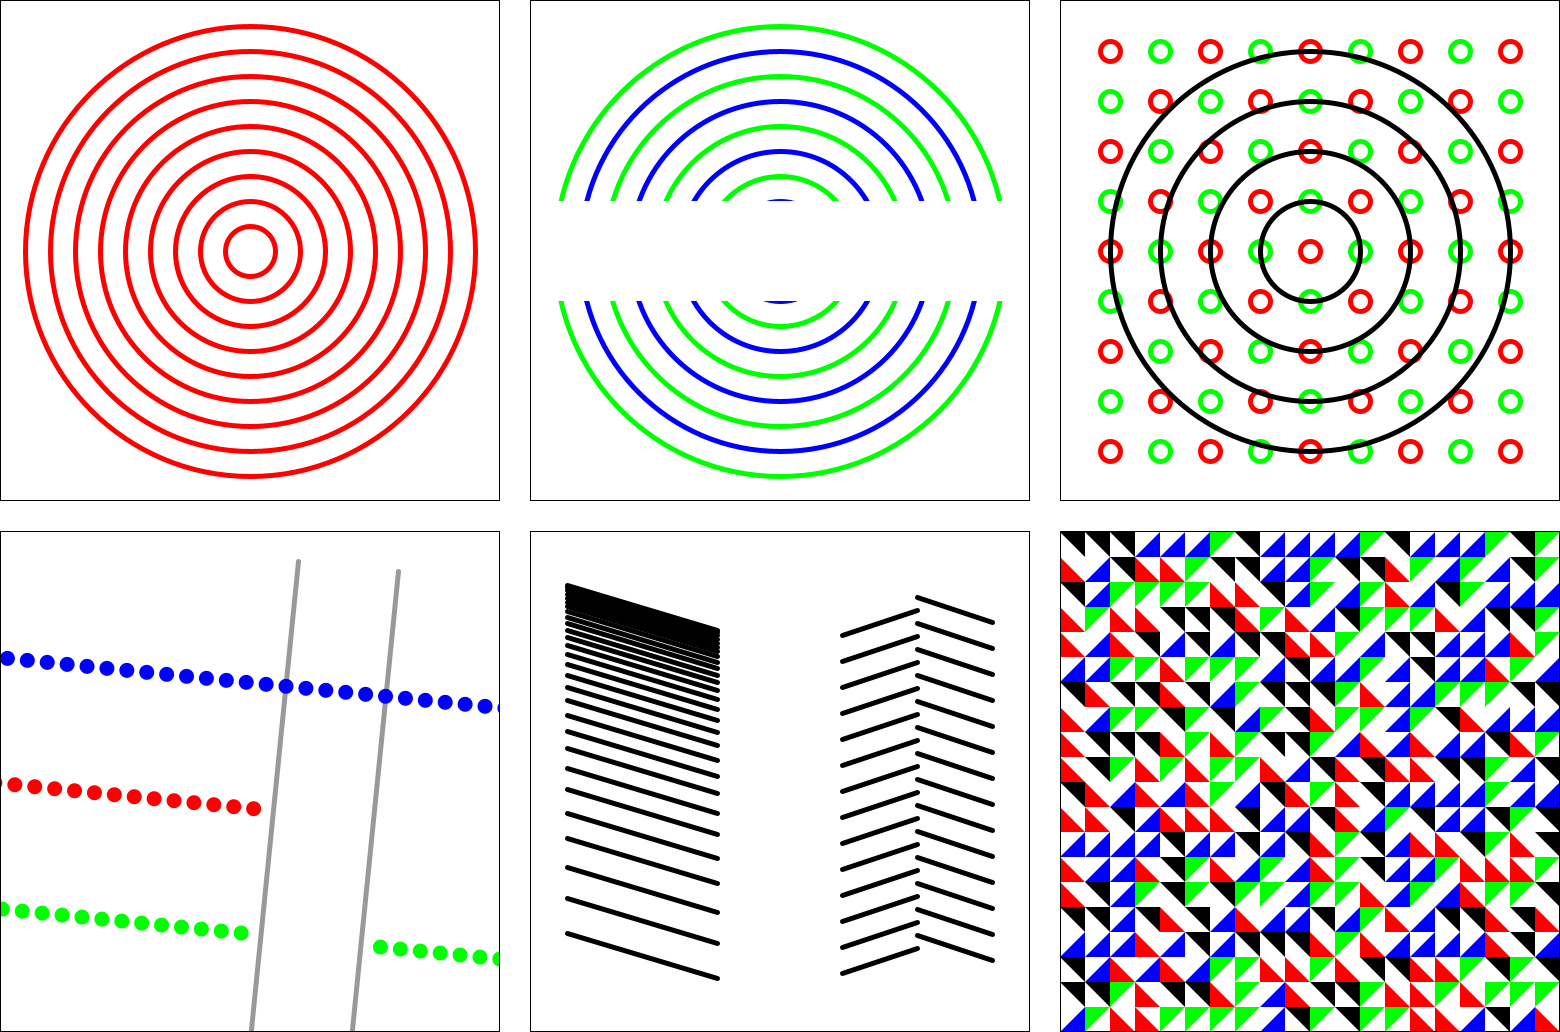
\includegraphics[width=1.0\textwidth]{chapters/chapter02-literature-review/tasks-challenges}
\caption{Thonny-py5mode graphical challenges. Developed by the author and implemented using py5. These graphics were used as prompts for various GenAI models to attempt reproduction.}
\label{fig:tasks-challenges}
\end{figure}

Someone with a reasonable understanding of Processing or py5 could likely outline a high-level approach to each task. While multiple approaches and code implementations could produce identical visual results, the intended solution path is apparent. To further support students, each task included starter code and contextual hints. For example, the top-left graphic included a scaffolded \texttt{while} loop and a comment indicating where to insert a red \texttt{stroke()} and a \texttt{circle()} function. Again, Appendix \ref{appendix:thonny-py5-mode-brief} contains the full Assessment~2 brief for the reader's reference.

Figures~\ref{fig:tasks-attempts-sonnet-4}, \ref{fig:tasks-attempts-2.5-flash}, and \ref{fig:tasks-attempts-gpt-4o} present the task attempts generated by Claude Sonnet 4, Gemini 2.5 Flash, and OpenAI GPT-4o, respectively. 

% pair and vertically center the first two attempts graphics
\begin{figure}[p]
  \vfill
  \centering
  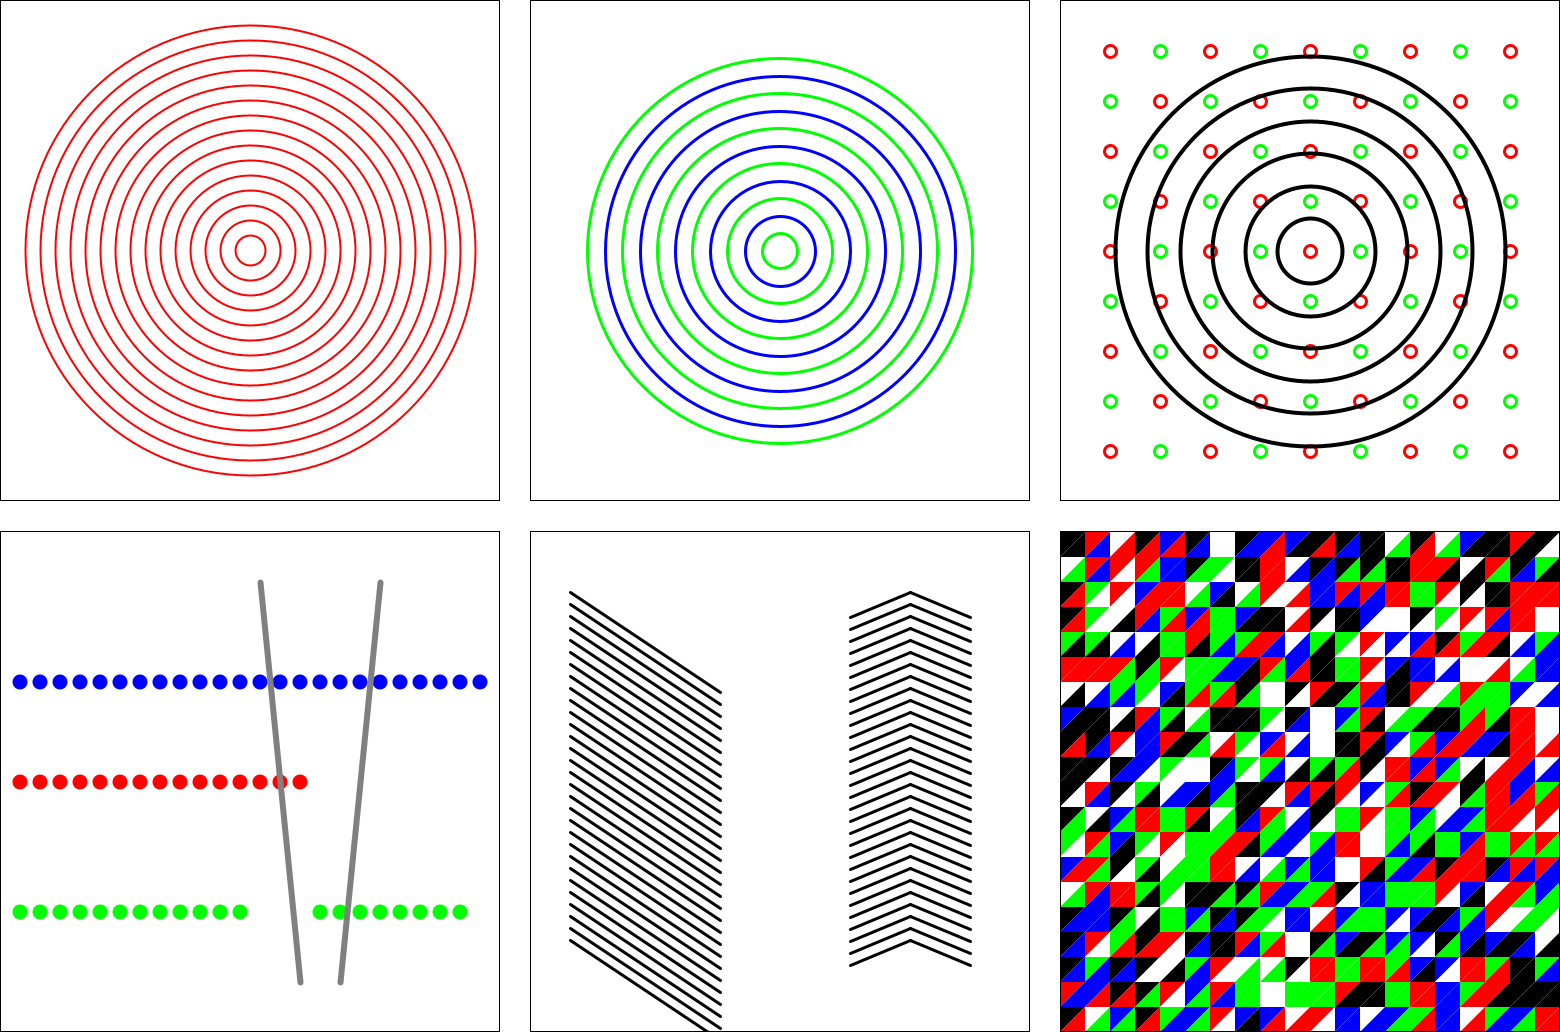
\includegraphics[width=0.8\textwidth]{chapters/chapter02-literature-review/tasks-attempts-sonnet-4}
  \caption{\textbf{Claude Sonnet 4} attempts at recreating the graphical challenges.}
  \label{fig:tasks-attempts-sonnet-4}

  \vspace{2em}
  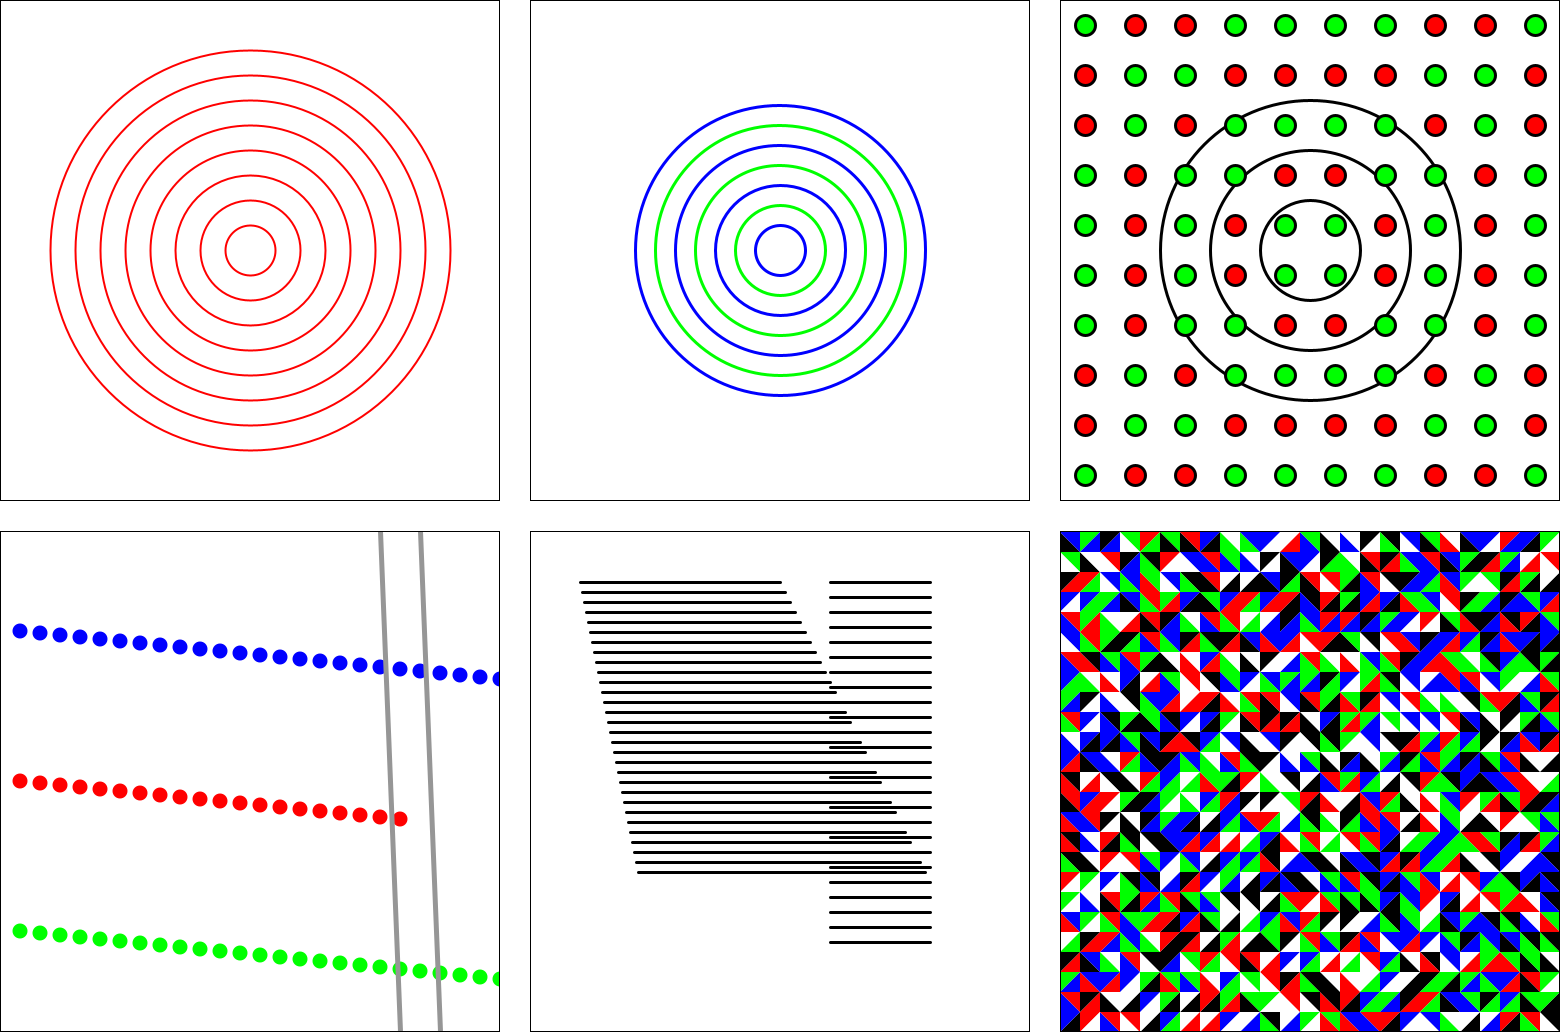
\includegraphics[width=0.8\textwidth]{chapters/chapter02-literature-review/tasks-attempts-2.5-flash}
  \caption{\textbf{Gemini 2.5 Flash} attempts at recreating the graphical challenges.}
  \label{fig:tasks-attempts-2.5-flash}
  \vfill
\end{figure}

\begin{figure}[H]%[htbp]
\centering

\includegraphics[width=0.8\textwidth]{chapters/chapter02-literature-review/tasks-attempts-gpt-4o}
\captionsetup{width=0.8\textwidth}
\caption{\textbf{OpenAI GPT-4o} attempts at recreating the graphical challenges.}
\label{fig:tasks-attempts-gpt-4o}
\end{figure}

For each model, the process involved uploading a single graphic at a time (e.g., the concentric red circles) to its chat interface, along with the corresponding starter code and a prompt requesting a py5-based solution. Of course, LLM outputs vary with each run. Figures~\ref{fig:tasks-attempts-sonnet-4}, \ref{fig:tasks-attempts-2.5-flash}, and \ref{fig:tasks-attempts-gpt-4o} display the closest result from three attempts per task, per model, with no follow-up prompts or corrections. As the reader can observe, inaccuracies range from relatively minor, such as a variance in the number of circles and stroke weight for the first (top left) task, to more conspicuous failures. For instance, none of the models identified that a white rectangle obscures the centre of the green-blue concentric circles (top row, middle graphic). The remaining outputs similarly fall short, often in ways that appear suspicious, as if a student approximated the layout and managed to code the tricky Python logic yet missed obvious visual characteristics.

\subsubsection{Future Work}

This preliminary exploration suggests that graphical programming tasks, especially those involving less prominent libraries, like py5, pose substantial challenges for current-generation LLMs. Despite receiving starter code and a clear visual target, prominent models consistently failed to produce accurate solutions---even after multiple attempts. These failures highlight a gap in GenAI capabilities: translating visual goals into functional graphical code, particularly when geometric precision or layered rendering is required.

Future work should investigate whether model performance improves with additional context, such as follow-up prompts and iterative refinement. It remains unclear whether explicitly providing such details, or even supplying relevant API documentation, would significantly improve results.

Alternative environments, such as p5.js or other Processing derivatives, warrant further investigation to determine whether more extensively documented libraries help mitigate LLM inaccuracy rates. However, some initial testing with Pillow (PIL) indicates that tasks requiring layered visual logic and spatial reasoning continue to pose significant challenges for GenAI models.

Introducing animation or dynamic behaviour could further increase difficulty, making it even harder for LLMs to generate correct code without human refinement. Additionally, the visual nature of such tasks lends itself to individualisation; instructors can algorithmically adjust parameters like position, colour, scale, or motion, thereby generating distinct variations of challenges for each student.

In some ways, these tasks echo the logic of CAPTCHA\footnote{~CAPTCHA systems are tests used to distinguish humans from bots using tasks like text recognition, image selection, or object manipulation~\cite{guerar_gotta_2022}. Think: squinting at blurry photos to find traffic lights and wondering if the one that appears in the corner of a tile counts.} systems: they rely on human perceptual judgement in ways machines still struggle to emulate. Research into this area may provide a deeper understanding to further exploit graphical tasks as a means of mitigating GenAI cheating. However, further research will require clearly defined criteria for assessing accuracy, particularly regarding what an appropriate grading rubric might entail and how to balance the emphasis between code quality and the fidelity of the visual output. Establishing such criteria would provide meaningful metrics for evaluating GenAI performance.

Ultimately, this line of inquiry invites further experimentation with prompt strategies, model capabilities, library familiarity, and individualised task generation. By designing assessments that deliberately probe the current limits of GenAI, educators can promote deeper student engagement while also mitigating the risk of superficial or unearned solutions.

\begin{description}[labelwidth=3.5em, leftmargin=!, labelindent=0pt]
\item[\colorbox{black}{\textcolor{white}{NOTE}}] On 2~September~2025, shortly before the completion of this thesis, Kiwi PyCon~2025 accepted a proposal arising from this line of enquiry, titled \textit{Mitigating AI Misuse in Introductory Python Courses with Graphical Programming Tasks}, for presentation in the academic track of the conference to be held 21--23~November in Wellington, New Zealand. As this was a late development, arising from research beyond the scope of this PhD, it is not included in the folio outputs.
\end{description}
